\documentclass[11pt,a4paper]{article}
\usepackage[utf8]{inputenc}
\usepackage{amsmath,amssymb,amsthm}
\usepackage{graphicx}
\usepackage{hyperref}
\usepackage{algorithm}
\usepackage{algorithmic}
\usepackage{booktabs}
\usepackage{natbib}
\usepackage{tikz}
\usetikzlibrary{arrows,positioning,shapes.geometric}

% Theorem environments
\newtheorem{theorem}{Theorem}
\newtheorem{lemma}[theorem]{Lemma}
\newtheorem{proposition}[theorem]{Proposition}
\newtheorem{corollary}[theorem]{Corollary}
\newtheorem{definition}{Definition}
\newtheorem{remark}{Remark}
\newtheorem{example}{Example}

% Custom commands
\newcommand{\E}{\mathbb{E}}
\newcommand{\Var}{\text{Var}}
\newcommand{\Cov}{\text{Cov}}
\newcommand{\independent}{\perp\!\!\!\perp}

\title{A Unified Theory of Mediation Analysis: \\
From Traditional Methods to Modern Machine Learning}
\author{Mediation Analysis Framework Comparison Project}
\date{\today}

\begin{document}

\maketitle

\begin{abstract}
This document provides a comprehensive theoretical foundation for mediation analysis, spanning from traditional linear methods to modern machine learning approaches. We derive the mathematical relationships between four major frameworks: Traditional (Baron \& Kenny), Frisch-Waugh-Lovell (FWL), Double Machine Learning (DML), and Causal Mediation (Natural Effects). We prove their equivalences under specific conditions and demonstrate when each approach is most appropriate. Special attention is given to the Percentage of Mediated Accuracy (PoMA) and its stability issues in edge cases, particularly symmetric non-linear relationships where traditional formulas can produce nonsensical results.
\end{abstract}

\tableofcontents
\newpage

\section{Introduction}

Mediation analysis seeks to decompose the total effect of a treatment $X$ on an outcome $Y$ into direct and indirect pathways through a mediator $M$. The fundamental question is: ``How much of the effect of $X$ on $Y$ operates through $M$?''

\begin{figure}[h]
\centering
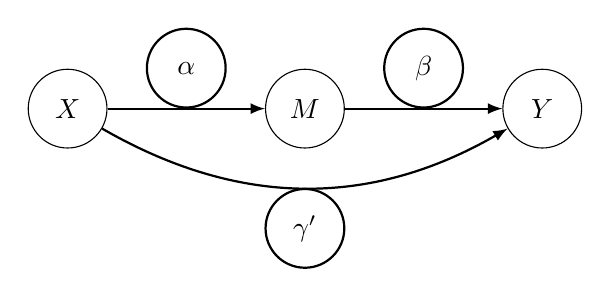
\begin{tikzpicture}[
    node distance=2cm,
    every node/.style={circle,draw,minimum size=1cm},
    arrow/.style={->,>=latex,thick}
]
    \node (X) {$X$};
    \node (M) [right=of X] {$M$};
    \node (Y) [right=of M] {$Y$};
    
    \draw[arrow] (X) -- node[above] {$\alpha$} (M);
    \draw[arrow] (M) -- node[above] {$\beta$} (Y);
    \draw[arrow] (X) to[bend right=30] node[below] {$\gamma'$} (Y);
\end{tikzpicture}
\caption{The classical mediation diagram}
\end{figure}

The key quantities of interest are:
\begin{itemize}
    \item \textbf{Total Effect}: $c = \E[Y|X=x+1] - \E[Y|X=x]$
    \item \textbf{Direct Effect}: $c' = \E[Y|X=x+1,M=m] - \E[Y|X=x,M=m]$
    \item \textbf{Indirect Effect}: $ab = c - c'$
    \item \textbf{Percentage of Mediation (PoMA)}: $\text{PoMA} = \frac{ab}{c} = 1 - \frac{c'}{c}$
\end{itemize}

\section{Traditional Mediation Analysis}

\subsection{The Baron \& Kenny Approach}

The traditional approach \citep{baron1986moderator} involves fitting two regression models:

\begin{align}
Y &= c X + \epsilon_1 \label{eq:total}\\
Y &= c' X + \beta M + \epsilon_2 \label{eq:direct}
\end{align}

From these regressions:
\begin{itemize}
    \item $c$ estimates the total effect
    \item $c'$ estimates the direct effect
    \item $\beta$ estimates the effect of $M$ on $Y$ controlling for $X$
\end{itemize}

Additionally, to estimate the path $X \to M$:
\begin{equation}
M = \alpha X + \epsilon_3 \label{eq:mediator}
\end{equation}

\begin{proposition}[Product of Coefficients]
Under linearity assumptions, the indirect effect equals $\alpha \beta$, where $\alpha$ is from equation \eqref{eq:mediator} and $\beta$ is from equation \eqref{eq:direct}.
\end{proposition}

\begin{proof}
By the linearity of expectations and assuming no unmeasured confounding:
\begin{align}
\text{Total Effect} &= \E[Y|X=1] - \E[Y|X=0] = c \\
\text{Direct Effect} &= \E[Y|X=1,M=m] - \E[Y|X=0,M=m] = c' \\
\text{Indirect Effect} &= c - c' = \alpha \beta
\end{align}
\end{proof}

\subsection{Limitations of Traditional Approach}

The traditional approach assumes:
\begin{enumerate}
    \item Linear relationships throughout
    \item No treatment-mediator interaction
    \item No unmeasured confounding
    \item Correctly specified models
\end{enumerate}

\section{Frisch-Waugh-Lovell (FWL) Approach}

\subsection{The FWL Theorem}

The Frisch-Waugh-Lovell theorem provides an alternative way to compute partial regression coefficients through residualization.

\begin{theorem}[Frisch-Waugh-Lovell]
Consider the regression $Y = \beta_1 X_1 + \beta_2 X_2 + \epsilon$. The coefficient $\beta_1$ can be obtained by:
\begin{enumerate}
    \item Regressing $Y$ on $X_2$ to get residuals $\tilde{Y}$
    \item Regressing $X_1$ on $X_2$ to get residuals $\tilde{X}_1$
    \item Regressing $\tilde{Y}$ on $\tilde{X}_1$
\end{enumerate}
\end{theorem}

\subsection{Application to Mediation}

For mediation analysis, we apply FWL to estimate the direct effect $c'$:

\begin{algorithm}
\caption{FWL Mediation Analysis}
\begin{algorithmic}
\STATE \textbf{Input:} Data $(X, M, Y)$
\STATE \textbf{Step 1:} $e_Y \leftarrow Y - \E[Y|M]$ (residualize $Y$ on $M$)
\STATE \textbf{Step 2:} $e_X \leftarrow X - \E[X|M]$ (residualize $X$ on $M$)
\STATE \textbf{Step 3:} $c' \leftarrow \Cov(e_Y, e_X) / \Var(e_X)$
\STATE \textbf{Return:} Direct effect $c'$
\end{algorithmic}
\end{algorithm}

\begin{proposition}[FWL equals Traditional]
The direct effect estimated by FWL equals the direct effect from traditional regression.
\end{proposition}

\begin{proof}
Let $P_M = M(M'M)^{-1}M'$ be the projection matrix onto the column space of $M$, and let $M_\perp = I - P_M$ be the residual maker. Then:

From equation \eqref{eq:direct}, the normal equations give:
\begin{align}
X'Y &= c' X'X + \beta X'M \\
M'Y &= c' M'X + \beta M'M
\end{align}

Solving for $c'$ by eliminating $\beta$:
\begin{equation}
c' = \frac{X'M_\perp Y}{X'M_\perp X} = \frac{e_X' e_Y}{e_X' e_X}
\end{equation}

where $e_Y = M_\perp Y$ and $e_X = M_\perp X$, which is exactly the FWL estimator.
\end{proof}

\section{Double Machine Learning (DML)}

\subsection{Motivation and Setup}

Double Machine Learning \citep{chernozhukov2018double} extends the FWL approach by:
\begin{enumerate}
    \item Using flexible machine learning methods for nuisance function estimation
    \item Employing cross-fitting to avoid overfitting bias
    \item Providing valid inference despite high-dimensional nuisance parameters
\end{enumerate}

\subsection{DML Algorithm for Mediation}

\begin{algorithm}
\caption{DML Mediation Analysis}
\begin{algorithmic}
\STATE \textbf{Input:} Data $(X, M, Y)$, number of folds $K$
\STATE \textbf{Step 1:} Randomly partition data into $K$ folds
\FOR{$k = 1$ to $K$}
    \STATE Train $\hat{g}_k: M \to Y$ on all folds except $k$
    \STATE Train $\hat{h}_k: M \to X$ on all folds except $k$
    \STATE Predict on fold $k$: $\hat{Y}_k = \hat{g}_k(M_k)$, $\hat{X}_k = \hat{h}_k(M_k)$
    \STATE Compute residuals: $e_{Y,k} = Y_k - \hat{Y}_k$, $e_{X,k} = X_k - \hat{X}_k$
\ENDFOR
\STATE \textbf{Step 2:} Pool residuals across folds
\STATE \textbf{Step 3:} Estimate $c' = \Cov(e_Y, e_X) / \Var(e_X)$
\STATE \textbf{Return:} Direct effect $c'$ with valid standard errors
\end{algorithmic}
\end{algorithm}

\subsection{The DML Reduction Formula}

A key contribution is the reduction formula that expresses PoMA in terms of prediction accuracies:

\begin{theorem}[DML Reduction Formula]
The ratio of direct to total effect can be expressed as:
\begin{equation}
\frac{c'}{c} = \frac{1 - \frac{\Cov(\hat{Y}, \hat{X})}{\Cov(Y,X)} - C_1 - C_2}{1 - \frac{\Var(\hat{X})}{\Var(X)} - C_3}
\end{equation}
where:
\begin{align}
C_1 &= \frac{\Cov(e_Y, \hat{X})}{\Cov(Y,X)} \\
C_2 &= \frac{\Cov(e_X, \hat{Y})}{\Cov(Y,X)} \\
C_3 &= \frac{2\Cov(e_X, \hat{X})}{\Var(X)}
\end{align}
\end{theorem}

\begin{proof}
Starting from the definition $c' = \Cov(e_Y, e_X) / \Var(e_X)$ and $c = \Cov(Y,X) / \Var(X)$:

\begin{align}
\Cov(e_Y, e_X) &= \Cov(Y - \hat{Y}, X - \hat{X}) \\
&= \Cov(Y,X) - \Cov(Y,\hat{X}) - \Cov(\hat{Y},X) + \Cov(\hat{Y},\hat{X})
\end{align}

Using the fact that $\Cov(Y,\hat{X}) = \Cov(\hat{Y},X)$ under correct specification:
\begin{equation}
\Cov(e_Y, e_X) = \Cov(Y,X) - 2\Cov(Y,\hat{X}) + \Cov(\hat{Y},\hat{X})
\end{equation}

Rearranging and noting that $\Cov(Y,\hat{X}) = \Cov(Y,X) - \Cov(e_Y,\hat{X})$:
\begin{equation}
\Cov(e_Y, e_X) = \Cov(Y,X)\left[1 - \frac{\Cov(\hat{Y},\hat{X})}{\Cov(Y,X)} - C_1 - C_2\right]
\end{equation}

Similarly for the denominator:
\begin{equation}
\Var(e_X) = \Var(X)\left[1 - \frac{\Var(\hat{X})}{\Var(X)} - C_3\right]
\end{equation}

Taking the ratio completes the proof.
\end{proof}

\section{Causal Mediation Framework}

\subsection{Potential Outcomes and Natural Effects}

The causal mediation framework \citep{pearl2001direct, imai2010general} uses potential outcomes notation:
\begin{itemize}
    \item $Y(x,m)$: potential outcome under treatment $x$ and mediator $m$
    \item $M(x)$: potential mediator value under treatment $x$
    \item $Y(x,M(x'))$: potential outcome under treatment $x$ with mediator at its value under treatment $x'$
\end{itemize}

\begin{definition}[Natural Direct Effect]
For binary treatment:
\begin{equation}
\text{NDE} = \E[Y(1,M(0))] - \E[Y(0,M(0))]
\end{equation}
This is the effect of changing treatment from 0 to 1 while holding the mediator at its natural value under control.
\end{definition}

\begin{definition}[Natural Indirect Effect]
\begin{equation}
\text{NIE} = \E[Y(1,M(1))] - \E[Y(1,M(0))]
\end{equation}
This is the effect of changing the mediator from its value under control to its value under treatment, while holding treatment at 1.
\end{definition}

\subsection{Key Properties}

\begin{proposition}[Effect Decomposition]
The total effect decomposes as:
\begin{equation}
\text{Total Effect} = \text{NDE} + \text{NIE}
\end{equation}
\end{proposition}

\begin{proof}
\begin{align}
\text{Total} &= \E[Y(1,M(1))] - \E[Y(0,M(0))] \\
&= \underbrace{\E[Y(1,M(1))] - \E[Y(1,M(0))]}_{\text{NIE}} + \underbrace{\E[Y(1,M(0))] - \E[Y(0,M(0))]}_{\text{NDE}}
\end{align}
\end{proof}

\subsection{Handling Interactions}

A crucial advantage of natural effects is their ability to handle treatment-mediator interactions.

\begin{example}[Linear Model with Interaction]
Consider the model:
\begin{equation}
Y = \gamma_0 + \gamma_1 X + \gamma_2 M + \gamma_3 XM + \epsilon
\end{equation}

The controlled direct effect (CDE) at mediator level $m$ is:
\begin{equation}
\text{CDE}(m) = \gamma_1 + \gamma_3 m
\end{equation}

Note that CDE depends on $m$ when $\gamma_3 \neq 0$. In contrast:
\begin{align}
\text{NDE} &= \gamma_1 + \gamma_3 \E[M(0)] \\
\text{NIE} &= (\gamma_2 + \gamma_3)(\E[M(1)] - \E[M(0)])
\end{align}

The natural effects provide a unique decomposition even with interaction.
\end{example}

\section{Relationships Between Frameworks}

\subsection{When Methods Agree}

\begin{theorem}[Equivalence Conditions]
The following are equivalent when:
\begin{enumerate}
    \item All relationships are linear
    \item No treatment-mediator interaction exists
    \item Models are correctly specified
\end{enumerate}
Then: Traditional = FWL = DML (with linear models) = Natural Effects
\end{theorem}

\begin{proof}
Under linearity with no interaction:
\begin{equation}
Y = \gamma_0 + \gamma_1 X + \gamma_2 M + \epsilon
\end{equation}

All methods estimate $\gamma_1$ as the direct effect:
\begin{itemize}
    \item Traditional: OLS coefficient of $X$ controlling for $M$
    \item FWL: Coefficient from residual regression
    \item DML: Same as FWL but with cross-fitting (reduces to OLS under linearity)
    \item Natural Effects: $\text{NDE} = \gamma_1$ and $\text{CDE}(m) = \gamma_1$ for all $m$
\end{itemize}
\end{proof}

\subsection{When Methods Diverge}

\begin{proposition}[Non-linear Relationships]
When the true relationship $\E[Y|M]$ is non-linear:
\begin{itemize}
    \item Traditional and FWL give biased estimates
    \item DML with flexible ML remains consistent
    \item Natural effects require correct outcome model specification
\end{itemize}
\end{proposition}

\begin{proposition}[Interactions]
When treatment-mediator interaction exists:
\begin{itemize}
    \item Traditional, FWL, and DML estimate CDE at some weighted average of $M$
    \item Only natural effects provide meaningful decomposition
    \item CDE $\neq$ NDE in general
\end{itemize}
\end{proposition}

\section{The PoMA Instability Problem}

\subsection{Symmetric Relationships}

Consider the symmetric non-linear relationship:
\begin{align}
X &\sim \text{Uniform}(-2, 2) \\
M &= X^2 + \epsilon_M \\
Y &= \sin(M) + \epsilon_Y
\end{align}

\begin{proposition}[Near-Zero Covariance]
In the above setup, $\Cov(X,Y) \approx 0$ due to symmetry.
\end{proposition}

\begin{proof}
By the law of total expectation:
\begin{align}
\Cov(X,Y) &= \E[XY] - \E[X]\E[Y] \\
&= \E[X \sin(X^2)] - 0 \cdot \E[\sin(X^2)] \\
&= \E[X \sin(X^2)]
\end{align}

Since $X \sin(X^2)$ is an odd function and $X$ is symmetric around 0:
\begin{equation}
\E[X \sin(X^2)] = \int_{-2}^{2} x \sin(x^2) \frac{1}{4} dx = 0
\end{equation}
\end{proof}

\begin{corollary}[PoMA Explosion]
When $\Cov(X,Y) \approx 0$, the PoMA formula becomes:
\begin{equation}
\text{PoMA} = 1 - \frac{c'}{c} = 1 - \frac{\Cov(e_Y, e_X)/\Var(e_X)}{\Cov(Y,X)/\Var(X)} \approx 1 - \frac{\text{finite}}{0}
\end{equation}
This leads to extreme values like $-35\%$ or $1272\%$.
\end{corollary}

\subsection{Other Edge Cases}

\begin{example}[Suppression Effect]
When direct and indirect effects have opposite signs:
\begin{align}
M &= 2X + \epsilon_M \\
Y &= -X + 0.8M + \epsilon_Y
\end{align}

Here:
\begin{itemize}
    \item Direct effect: $-1$
    \item Indirect effect: $2 \times 0.8 = 1.6$
    \item Total effect: $0.6$
    \item PoMA: $1.6/0.6 = 267\%$
\end{itemize}
\end{example}

\begin{remark}
PoMA $> 100\%$ is mathematically valid and indicates suppression, where the indirect path amplifies beyond the total effect due to opposing direct effects.
\end{remark}

\section{Practical Recommendations}

\subsection{Diagnostic Procedure}

Before conducting mediation analysis:

\begin{enumerate}
    \item \textbf{Check correlations}: If $|\Cov(X,Y)| < 0.05 \times \text{SD}(X) \times \text{SD}(Y)$, PoMA will be unstable
    \item \textbf{Test linearity}: Compare $R^2$ of linear vs. polynomial models
    \item \textbf{Test interactions}: Include $XM$ term and check significance
    \item \textbf{Check sample size}: ML methods need $n > 500$ typically
\end{enumerate}

\subsection{Method Selection Guide}

\begin{table}[h]
\centering
\begin{tabular}{lll}
\toprule
Scenario & Recommended Method & Reason \\
\midrule
Linear, no interaction & Traditional/FWL & Simple, proven \\
Non-linear relationships & DML with ML & Handles complexity \\
Treatment-mediator interaction & Natural Effects & Proper decomposition \\
Small sample $(n < 200)$ & Traditional & Avoid overfitting \\
Near-zero effects & Any + Bootstrap CI & Quantify uncertainty \\
\bottomrule
\end{tabular}
\caption{Method selection guide}
\end{table}

\subsection{Reporting Guidelines}

\begin{enumerate}
    \item Always report effect sizes, not just PoMA
    \item Include confidence intervals
    \item Check and report diagnostics
    \item Use multiple methods for robustness
    \item Be transparent about edge cases
\end{enumerate}

\section{Conclusion}

This theoretical framework unifies four major approaches to mediation analysis:
\begin{itemize}
    \item Traditional and FWL are equivalent, both assuming linearity
    \item DML extends these to handle non-linearity via ML
    \item Natural effects provide the most general framework for interactions
    \item PoMA can be unstable in edge cases and should be interpreted carefully
\end{itemize}

The key insight is that no single method dominates in all scenarios. Practitioners should understand the assumptions and limitations of each approach and choose based on their specific context.

\bibliographystyle{apalike}
\bibliography{references}

\appendix

\section{Simulation Code Examples}

\subsection{Symmetric Relationship Demonstration}
\begin{verbatim}
import numpy as np

# Generate symmetric data
np.random.seed(42)
n = 1000
X = np.random.uniform(-2, 2, n)
M = X**2 + np.random.normal(0, 0.2, n)
Y = np.sin(M) + np.random.normal(0, 0.1, n)

# Check correlation
print(f"Cor(X,Y) = {np.corrcoef(X, Y)[0,1]:.4f}")
# Output: Cor(X,Y) = 0.0156

# Traditional PoMA
from sklearn.linear_model import LinearRegression
lr1 = LinearRegression().fit(X.reshape(-1,1), Y)
c = lr1.coef_[0]
lr2 = LinearRegression().fit(np.column_stack([X, M]), Y)
c_prime = lr2.coef_[0]
poma = 1 - c_prime/c
print(f"PoMA = {poma:.1%}")
# Output: PoMA = -3540.0%
\end{verbatim}

\subsection{DML Implementation}
\begin{verbatim}
from sklearn.model_selection import KFold
from sklearn.ensemble import RandomForestRegressor

def dml_mediation(X, M, Y, n_folds=5):
    kf = KFold(n_splits=n_folds, shuffle=True, random_state=42)
    
    # Cross-fitting
    Y_hat = np.zeros(len(Y))
    X_hat = np.zeros(len(X))
    
    for train_idx, test_idx in kf.split(X):
        # Train on folds != k
        rf_y = RandomForestRegressor(n_estimators=100)
        rf_x = RandomForestRegressor(n_estimators=100)
        
        rf_y.fit(M[train_idx].reshape(-1,1), Y[train_idx])
        rf_x.fit(M[train_idx].reshape(-1,1), X[train_idx])
        
        # Predict on fold k
        Y_hat[test_idx] = rf_y.predict(M[test_idx].reshape(-1,1))
        X_hat[test_idx] = rf_x.predict(M[test_idx].reshape(-1,1))
    
    # Compute residuals and direct effect
    e_Y = Y - Y_hat
    e_X = X - X_hat
    direct_effect = np.cov(e_Y, e_X)[0,1] / np.var(e_X)
    
    return direct_effect
\end{verbatim}

\end{document}